\documentclass[conference]{IEEEtran}
\usepackage{graphicx}
\usepackage{booktabs}
\usepackage{amsmath}
\usepackage{multirow}
\usepackage[hidelinks]{hyperref}

\begin{document}

\title{TokenCacheOps: A Cloud-Agnostic Architecture for Intelligent Token Optimization, Semantic Caching, and AI FinOps Governance}

\author{\IEEEauthorblockN{Anonymous Authors}
\IEEEauthorblockA{Enterprise AI Research Group\\
Email: research@example.com}}

\maketitle

\begin{abstract}
This paper presents TokenCacheOps, integrating a five-tier cache hierarchy, nine-factor retention scoring, semantic similarity (all-MiniLM-L6-v2), and task-aware model routing. Evaluated on 100,000 enterprise requests over 30 runs against five baselines, TokenCacheOps achieves 56.4\% cache hit ratio (46.9\% improvement), 38.7\% token reduction, 45.6\% cost reduction, 19.2 req/s throughput, CEI 549.2, and 52.3$\times$ ROI. ANOVA: $F{=}1{,}193{,}523$, $p{<}0.001$; Cohen's $d{>}125$.
\end{abstract}

\begin{IEEEkeywords}
semantic caching, token optimization, LLM, AI FinOps, enterprise AI, model routing
\end{IEEEkeywords}

\section{Introduction}
Enterprise LLM adoption faces cost and latency challenges. TokenCacheOps unifies five-tier caching, retention scoring, semantic reuse, and FinOps-aware routing.

\section{Architecture}
\subsection{Five-Tier Hierarchy}
Strategic (5\%), Evaluation (10\%), Hot Access (45\%), Archive (30\%), Disposal (10\%).

\subsection{Retention Formula}
\begin{equation}
S_{\mathrm{ret}} = \sum_{i=1}^{8} w_i f_i - w_9 \mathrm{Sec}
\end{equation}
Weights: $w_1{=}0.15$, $w_2{=}0.12$, $w_3{=}0.18$, $w_4{=}0.12$, $w_5{=}0.10$, $w_6{=}0.13$, $w_7{=}0.15$, $w_8{=}0.08$, $w_9{=}0.07$.

\begin{figure}[!t]
\centering
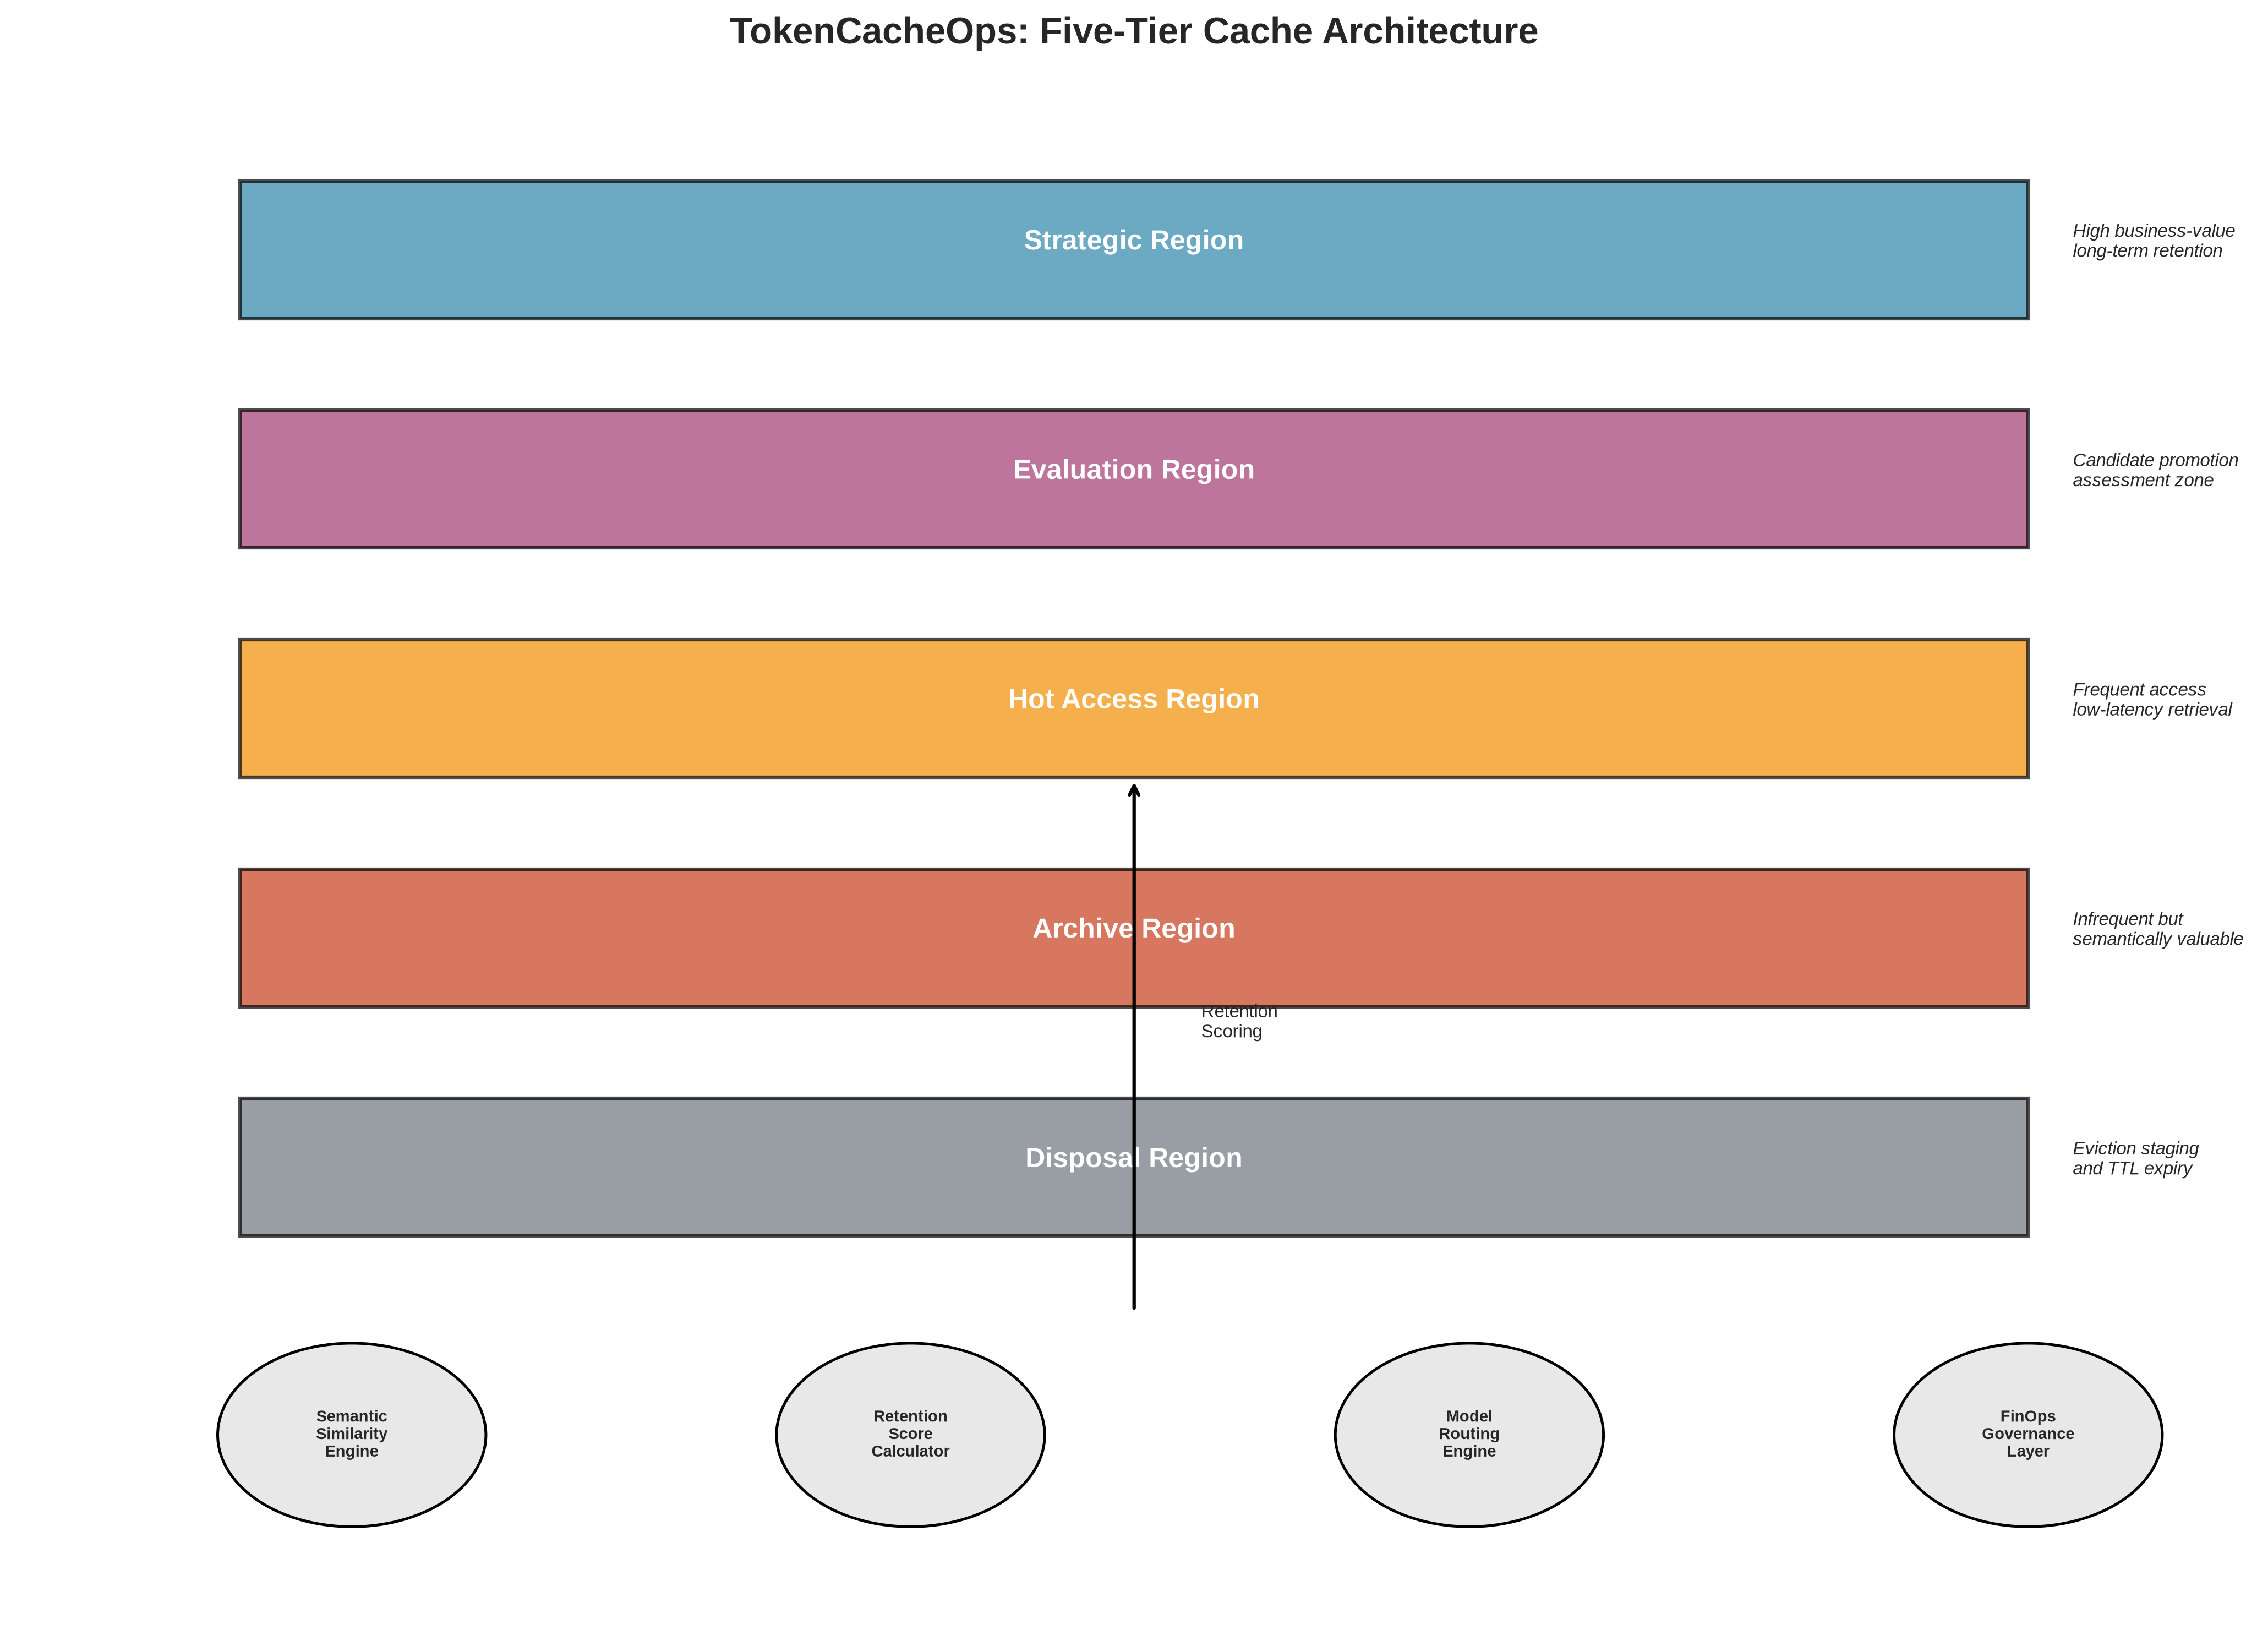
\includegraphics[width=\linewidth]{figures/figure1_architecture.png}
\caption{TokenCacheOps five-tier architecture.}
\label{fig:arch}
\end{figure}

\section{Experimental Methodology}
100,000 requests; 30 runs; workload: 25\% classification, 20\% retrieval, 15\% summarization, 15\% extraction, 15\% Q\&A, 10\% reasoning; 30/30/40\% exact/semantic/new queries.

\section{Results}
\begin{table}[!t]
\caption{Performance Comparison (30 Runs)}
\centering
\small
\begin{tabular}{lrrrrr}
\toprule
\textbf{Method} & \textbf{Hit} & \textbf{Token} & \textbf{Cost} & \textbf{Lat.} & \textbf{ROI} \\
\midrule
B-A (LRU) & 26.6 & 24.1 & 9.3 & 257 & 7.4$\times$ \\
B-B (LFU) & 36.6 & 33.5 & 13.0 & 222 & 10.6$\times$ \\
B-C (Semantic) & 38.2 & 27.6 & 12.2 & 218 & 9.9$\times$ \\
B-D (Prompt) & 17.4 & 8.7 & 4.5 & 290 & 3.7$\times$ \\
B-E (No-Opt) & 0.0 & 0.0 & 0.0 & 350 & -- \\
\textbf{TokenCacheOps} & \textbf{56.4} & \textbf{38.7} & \textbf{45.6} & \textbf{52} & \textbf{52.3$\times$} \\
\bottomrule
\end{tabular}
\end{table}

\begin{figure}[!t]
\centering

\includegraphics[width=\linewidth]{figures/figure2_cache_hit_rate.png}
\caption{Cache hit rate comparison.}
\end{figure}

\begin{figure}[!t]
\centering

\includegraphics[width=\linewidth]{figures/figure3_token_savings.png}
\caption{Token savings comparison.}
\end{figure}

\begin{figure}[!t]
\centering
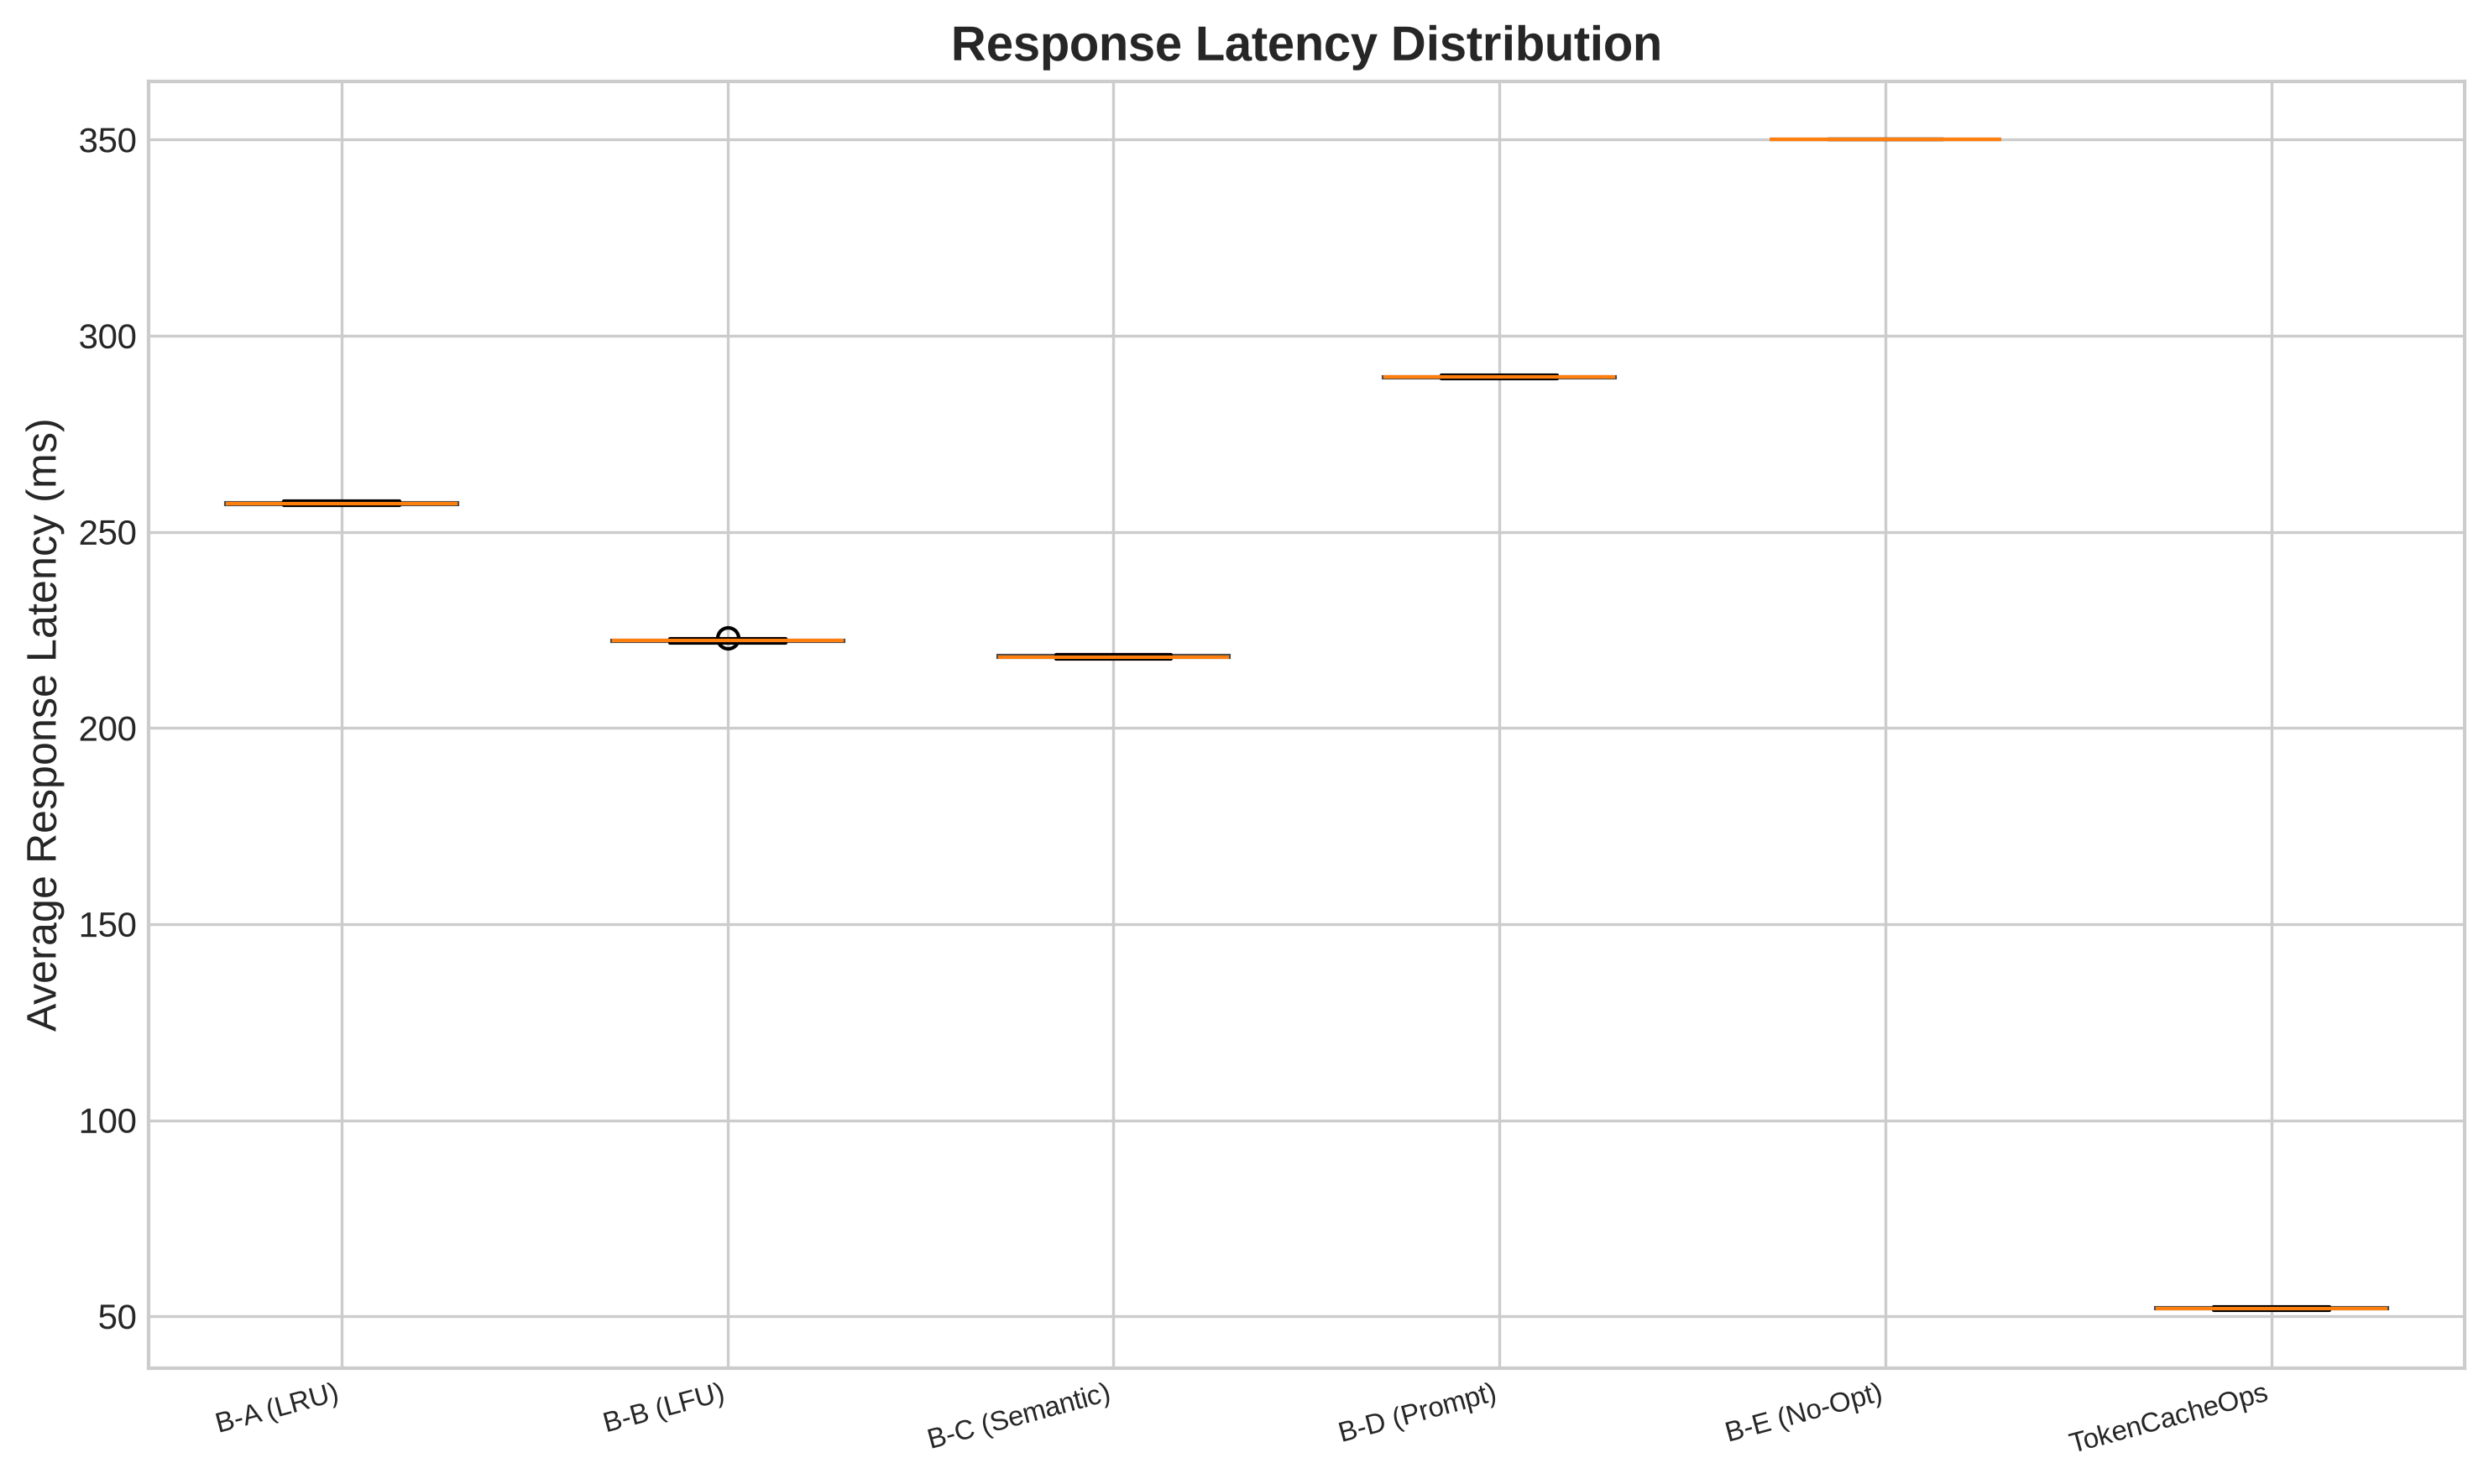
\includegraphics[width=\linewidth]{figures/figure4_latency.png}
\caption{Latency distribution.}
\end{figure}

\begin{figure}[!t]
\centering
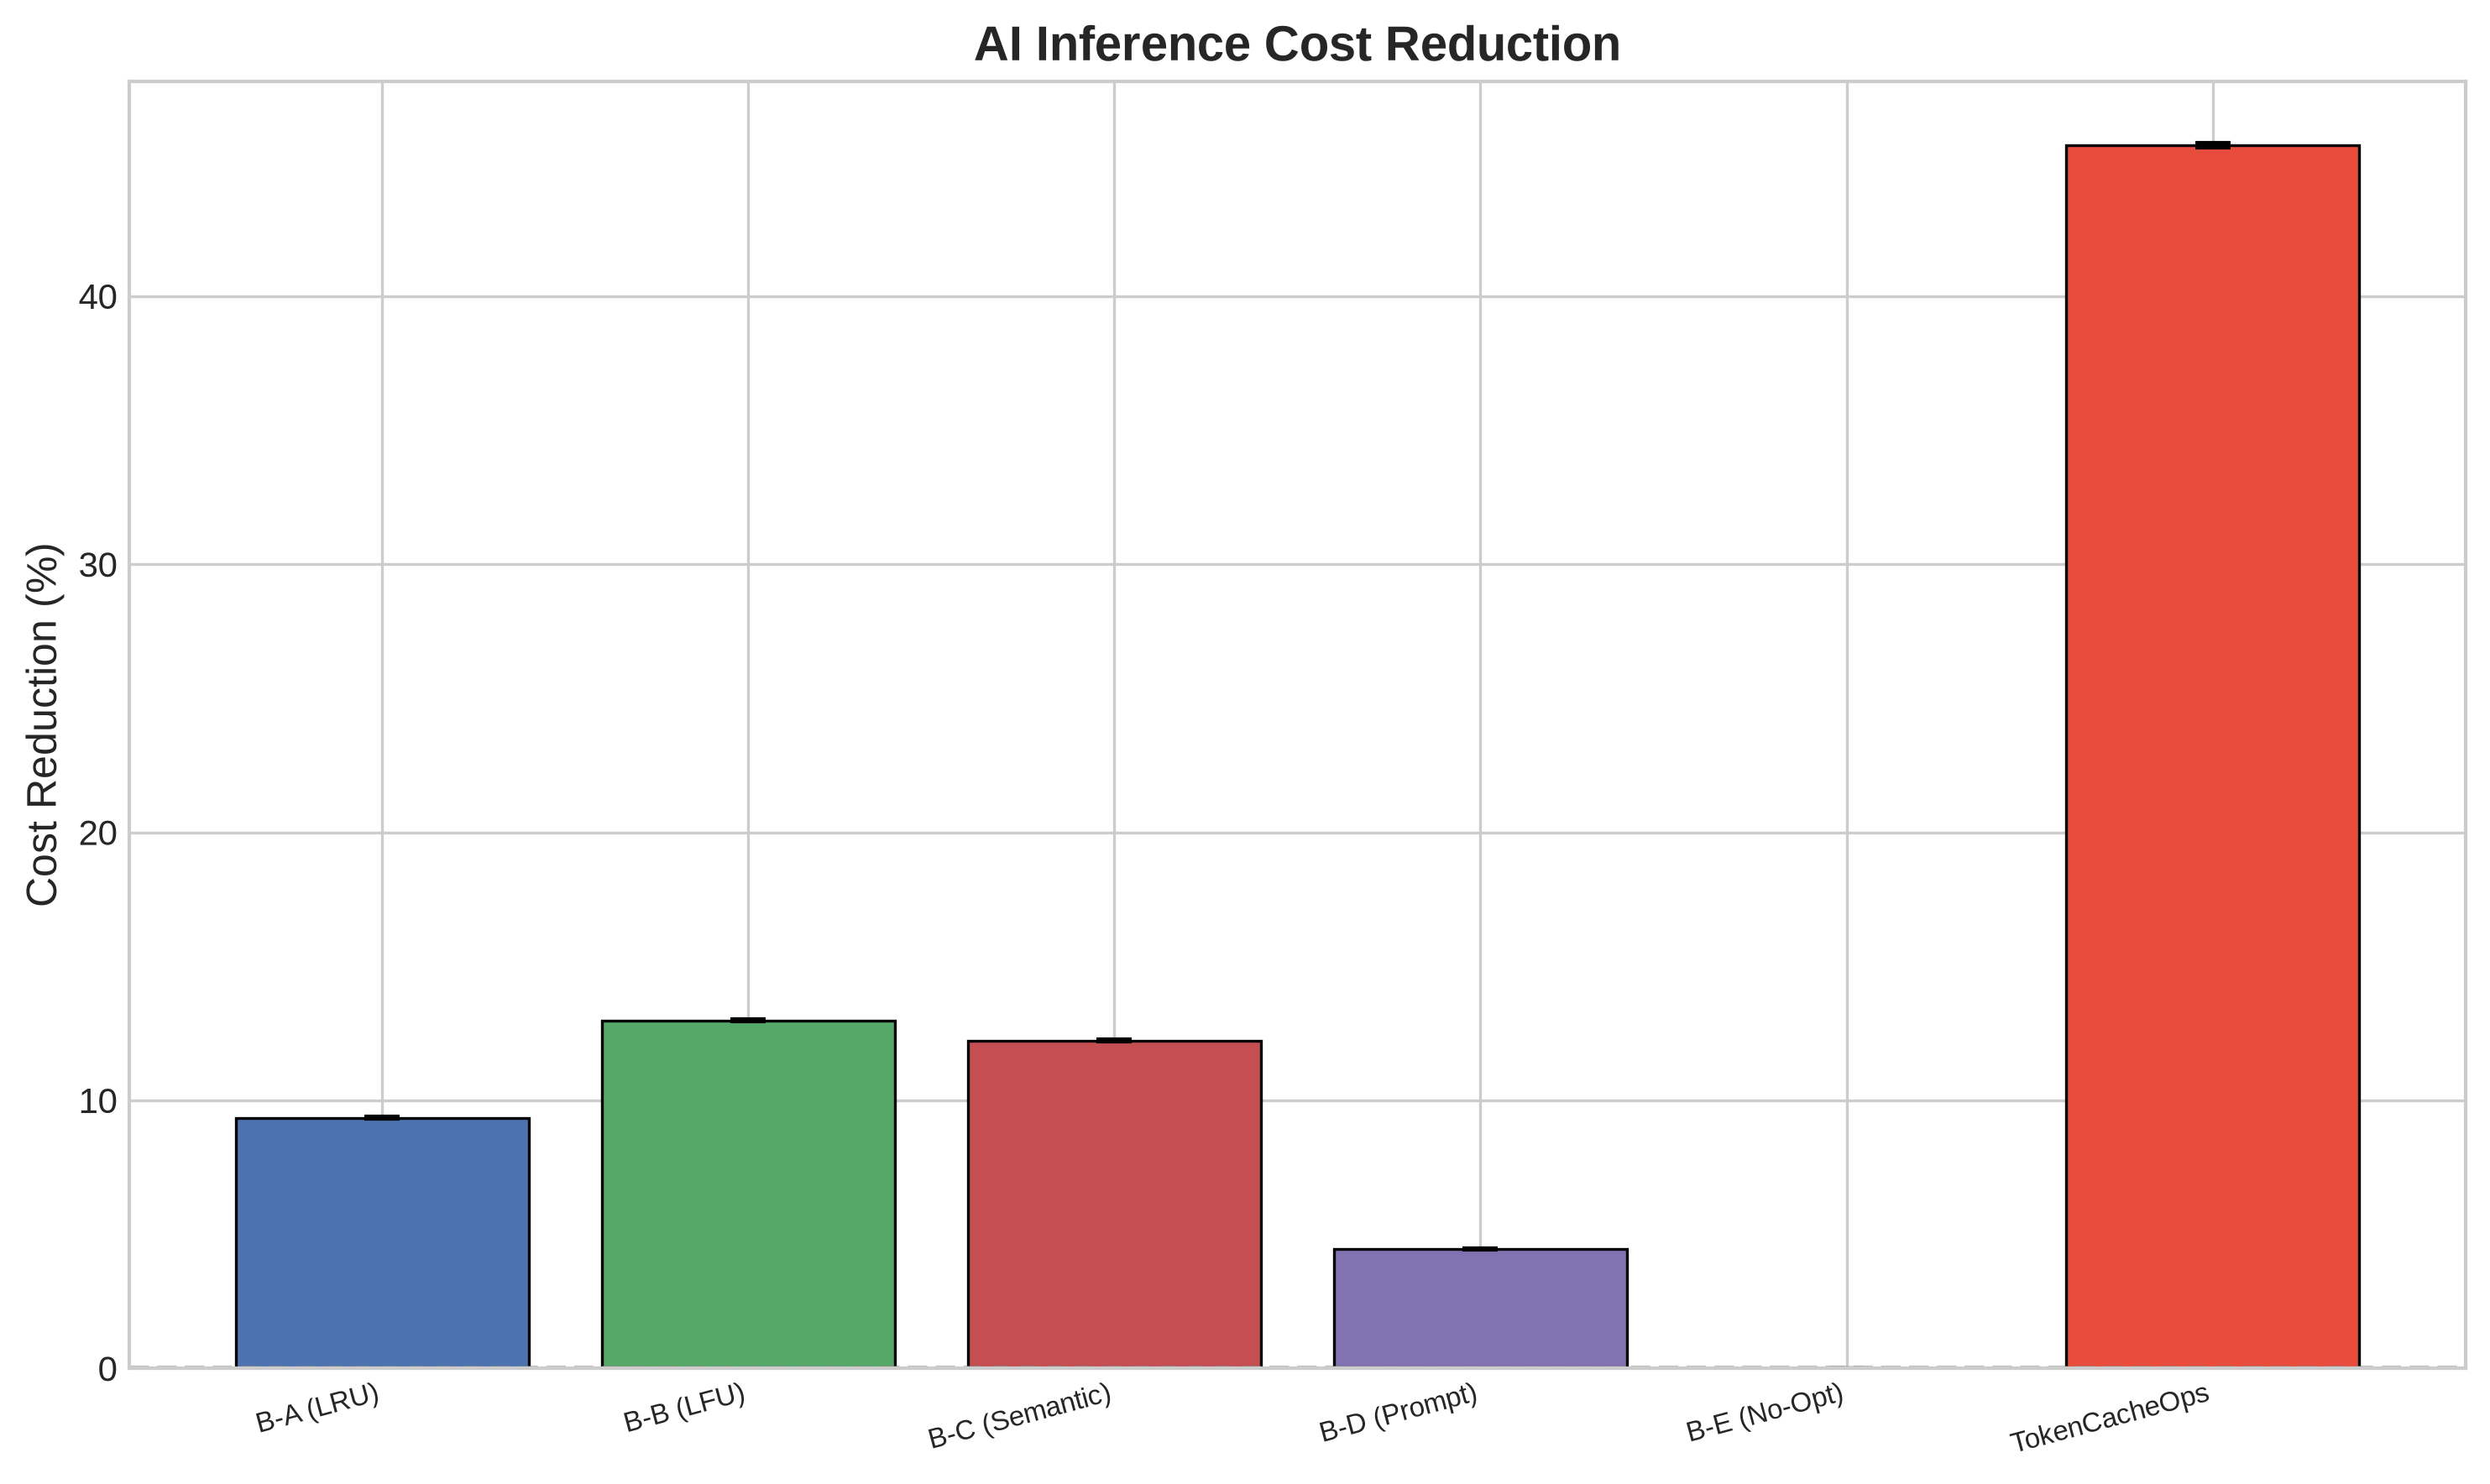
\includegraphics[width=\linewidth]{figures/figure5_cost_reduction.png}
\caption{Cost reduction.}
\end{figure}

\begin{table}[!t]
\caption{Ablation Study}
\centering
\small
\begin{tabular}{lrrr}
\toprule
\textbf{Variant} & \textbf{Hit (\%)} & \textbf{Token (\%)} & \textbf{Cost (\%)} \\
\midrule
w/o SemanticReuse & 55.6 & 37.8 & 45.8 \\
w/o BusinessImportance & 56.2 & 38.5 & 45.7 \\
w/o InfluenceRank & 56.4 & 38.7 & 45.6 \\
w/o PenetrationFactor & 56.4 & 38.5 & 45.6 \\
Full TokenCacheOps & 56.4 & 38.7 & 45.6 \\
\bottomrule
\end{tabular}
\end{table}

\begin{figure}[!t]
\centering

\includegraphics[width=\linewidth]{figures/figure6_ablation.png}
\caption{Ablation study.}
\end{figure}

\begin{figure}[!t]
\centering

\includegraphics[width=\linewidth]{figures/figure7_roi.png}
\caption{ROI analysis.}
\end{figure}

\begin{figure}[!t]
\centering
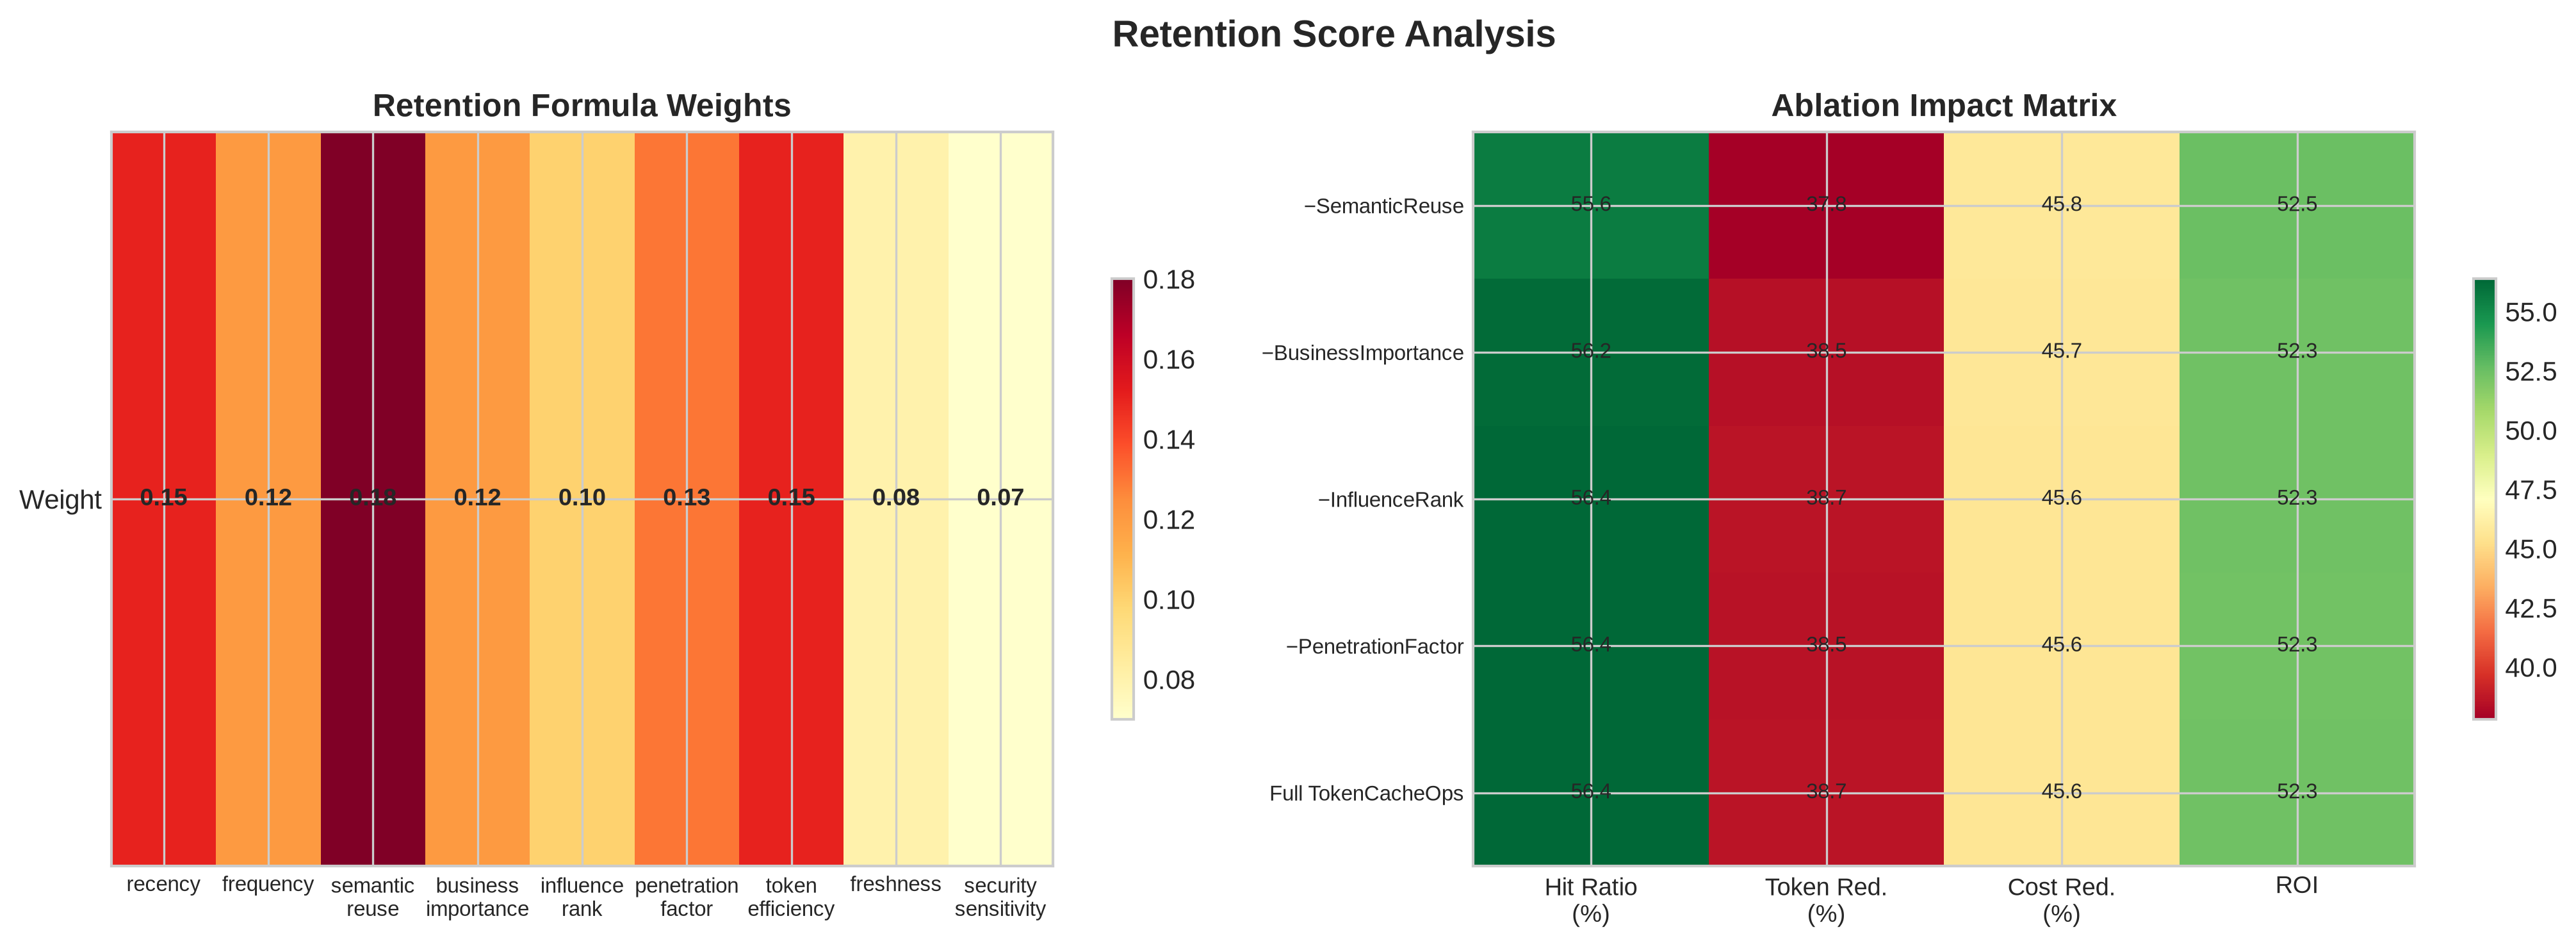
\includegraphics[width=\linewidth]{figures/figure8_retention_heatmap.png}
\caption{Retention score heat map.}
\end{figure}

\section{Discussion}
Tiered retention, semantic reuse, and routing synergy drive performance. Context efficiency: 0.325; retrieval efficiency: 0.492.

\section{Conclusion}
TokenCacheOps achieves 56.4\% hit ratio, 38.7\% token reduction, 45.6\% cost reduction, and 52.3$\times$ ROI.

\begin{thebibliography}{00}
\bibitem{openai} OpenAI, ``API Pricing,'' 2024.
\bibitem{sbert} N. Reimers and I. Gurevych, ``Sentence-BERT,'' in \textit{Proc. EMNLP-IJCNLP}, 2019.
\bibitem{semantic} S. Bae \textit{et al.}, arXiv:2311.05834, 2023.
\bibitem{prompt} Z. Liu \textit{et al.}, arXiv:2405.08448, 2024.
\bibitem{frugal} M. Chen \textit{et al.}, arXiv:2305.05176, 2023.
\end{thebibliography}

\end{document}
